\documentclass[a4paper,11pt]{kth-mag}
\usepackage[T1]{fontenc}
\usepackage{textcomp}
\usepackage{lmodern}
\usepackage[latin1]{inputenc}
\usepackage[swedish,english]{babel}
\usepackage{modifications}
\usepackage[backend=bibtex]{biblatex}
% code
\usepackage{listings}
\usepackage{color}

\usepackage{minted}

\usepackage{graphicx}

\usepackage{caption}

\newcommand{\codesize}{\footnotesize}

\pdfoptionpdfminorversion 6

\bibliography{bib/database.bib}

\definecolor{dkgreen}{rgb}{0,0.6,0}
\definecolor{gray}{rgb}{0.5,0.5,0.5}
\definecolor{mauve}{rgb}{0.58,0,0.82}

\lstset{frame=tb,
  language=Java,
  aboveskip=3mm,
  belowskip=3mm,
  showstringspaces=false,
  columns=flexible,
  basicstyle={\small\ttfamily},
  numbers=none,
  keywordstyle=\color{blue},
  commentstyle=\color{dkgreen},
  stringstyle=\color{mauve},
  breaklines=true,
  breakatwhitespace=true
  tabsize=3
}


\title{A Reactive platform for Data Integration and Event Stream Processing}

\subtitle{Duis autem vel eum iruire dolor in hendrerit in
          vulputate velit esse molestie consequat, vel illum
          dolore eu feugiat null}
\foreigntitle{Lorem ipsum dolor sit amet, sed diam nonummy nibh eui
              mod tincidunt ut laoreet dol}
\author{Namn Namnet}
\date{November 2003}
\blurb{Master's Thesis at NADA\\Supervisor: Tjoho\\Examiner: Tjohej}
\trita{TRITA xxx yyyy-nn}
\begin{document}
\frontmatter
\pagestyle{empty}
\removepagenumbers
\maketitle
\selectlanguage{english}

\begin{abstract}
  This is a skeleton for KTH theses. More documentation
  regarding the KTH thesis class file can be found in
  the package documentation.

Lorem ipsum dolor sit amet, consectetuer adipiscing elit. Mauris
purus. Fusce tempor. Nulla facilisi. Sed at turpis. Phasellus eu
ipsum. Nam porttitor laoreet nulla. Phasellus massa massa, auctor
rutrum, vehicula ut, porttitor a, massa. Pellentesque fringilla. Duis
nibh risus, venenatis ac, tempor sed, vestibulum at, tellus. Class
aptent taciti sociosqu ad litora torquent per conubia nostra, per
inceptos hymenaeos.
\end{abstract}

\clearpage

\begin{foreignabstract}{swedish}
  Denna fil ger ett avhandlingsskelett.
  Mer information om \LaTeX-mallen finns i
  dokumentationen till paketet.

Lorem ipsum dolor sit amet, consectetuer adipiscing elit. Maurisd
purus. Fusce tempor. Nulla facilisi. Sed at turpis. Phasellus eu
ipsum. Nam porttitor laoreet nulla. Phasellus massa massa, auctor
rutrum, vehicula ut, porttitor a, massa. Pellentesque fringilla. Duis
nibh risus, venenatis ac, tempor sed, vestibulum at, tellus. Class
aptent taciti sociosqu ad litora torquent per conubia nostra, per
inceptos hymenaeos.
\end{foreignabstract}
\clearpage
\tableofcontents*

\mainmatter
\pagestyle{newchap}

\chapter{Introduction}

\section{Context and system overview}

Data is now at the center of organizations and is increasingly heterogeneous with an explosion of data sources 
that each exposes data in its own format that can be structured, semi-structured or non-structured.
Another major trend is that data processing needs to be real-time, because business men no longer want to wait a whole day 
to have reports and alerts on their business data. Last but not least, the volume of data that enterprises need to analyze is constantly growing, which is commonly referred as "Big Data".
\\

To achieve these requirements, traditional monolithic Data Wharehouse softwares start to be out-dated. They often
propose to deal only with structured data to map it to a relational model, and are often batch-oriented: 
the ETL mechanism (data extraction, transform and load) regularly happens once or twice per day, and there is no mechanism 
for real-time subscriptions on new events happening on the data (as highlighted by Jay Kreps, engineer at LinkedIn, 
in his article "The Log: What every software engineer should know about real-time data's unifying abstraction" \footfullcite{bib:linkedinLog}). Moreover,
Data Integration, Data Storage and Data Reporting are often coupled into a single monolithic software.
\\

Thus, a new kind of architecture for Data Integration and Data Processing is needed in order to meet these new requirements: real-time processing of potentially big volumes of unstructured data. This thesis presents an architecture that solves this problem using \textit{decoupled components} that communicate with \textit{immutable events} that represent data changes. Events flow across the platform enabling components to react to data changes in various ways. Real-time should be understood as \textit{soft} real-time in comparison to batch modes that are more common in Big Data frameworks. For example, event propagation across the platform should be measured in milliseconds or seconds, whereas batch jobs are often measured in hours. Moreover, in a real-time platform, the notion of Big Data is more related to the push rate of events than the size of an event itself. Thus, the platform should take care of possible performance problems in order to handle high push rates.

Each event represents the change (creation, update or deletion) made to a data resource at a particular time. Based on the Event-Sourcing principle \footfullcite{bib:eventSourcing}, events are stored in a Journal that is an ordered sequence of events. Then, the stream of events coming from the Journal can be processed by data consumers that can react to the change of data (see Figure \ref{fig:main_archi} for the global architecture). 
An example of data consumer can be one that maintains a pre-computed view on the data that is updated upon each event, or one that pushes 
notifications to another service upon the reception of some kinds of events.
\\

An example use case is when an organization uses different SaaS services for each of its teams. For instance, the sales
team uses a SaaS software to process their sales pipeline, the project management team uses another SaaS software to manage
the production teams, etc... Without a central data backbone, it is not possible to have a global view on the company data.
The platform I present in this thesis can integrate these different SaaS softwares using their REST API, detect what
changes have been made on the data, and emit the corresponding events. As a result, data consumers can use these events
to update dashboards about the company data in real-time, mixing the data coming from different sources. A data consumer can also push a
notification to SaaS service X when it receives an event from SaaS service Y, allowing real-time synchronization between
heterogeneous services.
\\

An advantage of Event Sourcing is that the whole history of the system is stored. Events are immutable changes made to the data
and are always appended to the Journal (never deleted or modified). As a result, the system stores not only the current state
of the data, but also all its previous states. This allows two interesting properties.

First, it is possible to query past states of the data. This can be very useful for various use cases
where one is interested in the data history, for example a financial audit.

Moreover, storing all the data changes greatly improves the fault-tolerance of the system. As events are not deleted, it is always possible 
to come back in the past in the Journal, delete some delete events that were put by mistake, and replay the events after
them to re-build the system in a right state. This is also referred as Human Fault-Tolerance \footfullcite{bib:human-ft}: in a mutable system,
if an user accidentally delete a data entry, it is lost for ever. But in an immutable system, the deletion is just another
event added to the journal. Figure \ref{fig:event-sourcing} illustrates the difference between a mutable system and an immutable event-sourced system.
\\ 

\begin{figure}[h]
  \begin{center}
    \makebox[\textwidth]{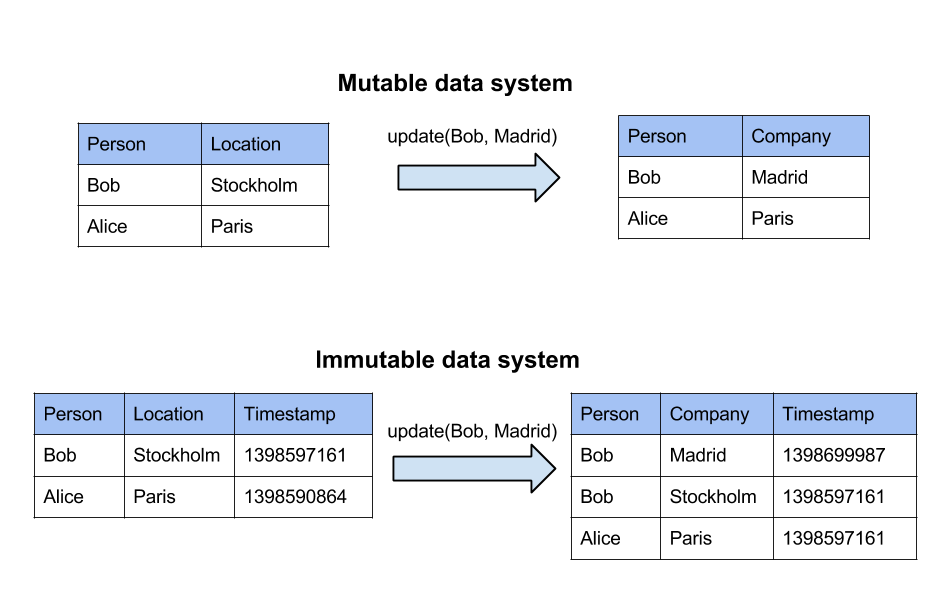
\includegraphics[width=1.0\textwidth]{img/event-sourcing.png}}
    \caption{Immutable datastore and the Event Sourcing principle}
    \label{fig:event-sourcing}
  \end{center}
\end{figure}

This kind of architecture is also known as CQRS \footfullcite{bib:cqrs}. The core principle of CQRS is to decouple the write part and the read part
of a system. The write part (Data Integration) only needs to push immutable events to the Journal in an append-only fashion, which
is very efficient because there is no mutation of the data and no read-write contentions as in traditional databases.
The read part is a set of denormalized pre-computed views that are optimized for low read latency (as the views are automatically re-computed
when a new related event comes in).
An obvious downside of such an architecture is that data is eventually consistent: when a data producer has received the acknowledgment
from the Journal, there is no guarantee that data consumers has already processed the event and updated the data view.

This model also allows very easy distribution of the platform because it enables a message-oriented
architecture where each component (data producer, journal, data consumers with data views) only exchanges messages (events) with each other (share-nothing architecture).
\\

The platform is composed of three main parts: 
\begin{itemize}
  \item Data Integration, that must integrate several data sources in order to emit 
events (data changes) to the Journal. 
  \item Journal, an abstraction for a sequence of immutable events. The Journal must expose methods to insert events,
  and expose methods to subscribe to the stream of events.
  \item Stream processing, where one can define a tree of data consumers (stream processors) that can react to
  events, maintain derived pre-computed views on the data, and emit new streams of events.
\end{itemize}

\begin{figure}[h]
  \begin{center}
    \makebox[\textwidth]{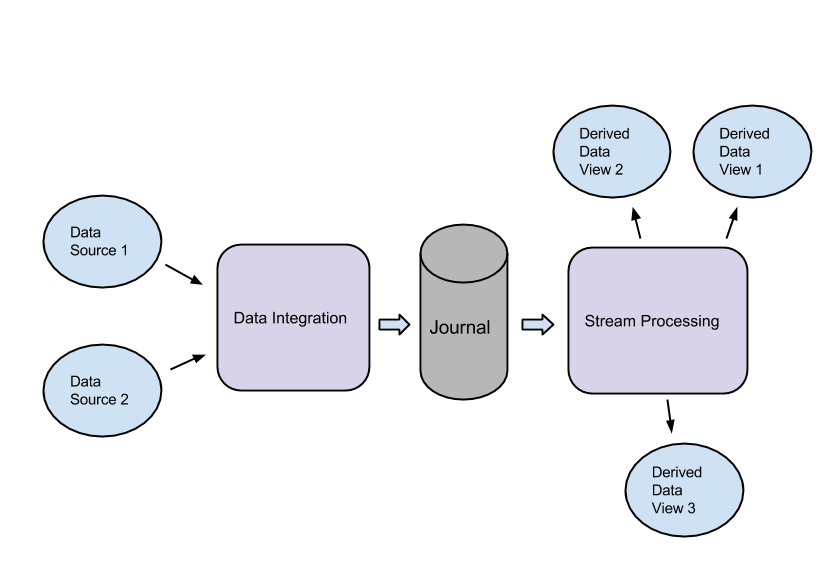
\includegraphics[width=1.0\textwidth]{img/main_archi.png}}
    \caption{Global architecture}
    \label{fig:main_archi}
  \end{center}
\end{figure}

Nonetheless, this kind of evented architecture must be done with a lot of care concerning technical architecture.
The platform needs to do lot of IO in order to push the stream of events from data sources to data consumers, and must
parallelize a lot of operations. Moreover, it must ensure that the stream of events (producers) does not overwhelm the stream
processors (consumers), i.e. if consumers process data slowly, producers must try to slow the push rate. The platform should also deal with possible
failures of components and offer strong guarantees in these cases (like no message loss or duplication).

In order to fulfill those requirements, the platform will apply the principles of the Reactive Manifesto \footfullcite{bib:reactiveManifesto} in order to guarantee
that the platform is \textit{scalable, event-driven, resilient and responsive} (the four Reactive Traits). An asynchronous non-blocking approach with a share-nothing architecture will be used to develop the platform in order to optimize resource consumption, decouple components to be able to distribute them easily, take easily advantage of parallelization and handle failures. 
The platform is developed using functional programming in the Scala programming language \footfullcite{bib:scala} in order to leverage functional programming abstractions to better handle asynchronous and stream-oriented code.
\\


\section{Related works}

There exists several Big Data frameworks for real-time processing. Among them, Apache Kafka \footfullcite{bib:kafka} and Apache Storm \footfullcite{bib:stormframework} have been thoroughly studied for this thesis.
\\

Apache Kafka is a high-throughput distributed messaging system developed at LinkedIn. It is a distributed publish-subscribe system where data producers can send messages in topics and data consumers can subscribe to topics. It is durable by persisting messages on disk and data consumers can pull events with a guaranteed order. However, as it uses a publish-subscribe abstraction, it does not enable the user to define clear stream processing flow structures (such as trees or DAGs) where components are both data consumers (receiving events from parent components) and data producers (sending events to their child components).
\\

Apache Storm is a distributed and fault-tolerant real-time computation framework developed at Twitter. It enables the user to define a DAG of stream processors that can receive event from their parent(s) and send derived events to their children. However, messages are not persisted on disk, so there is no durability, which implies that slow processors are forced to keep past events in-memory if we want fast processors to move on to next events without waiting for slow processors (more details will be given on these types of recurrent stream processing issues in chapter \ref{chapt:streamproc}).
\\

As explained in more details in the thesis, our platform will take some architecture patterns of these two frameworks to achieve an original architecture with a list of properties that none of these frameworks fully provide on their own.

\section{Contributions}

The main contributions of this thesis are:
\begin{itemize}
  \item Definition of the architecture of the Data Integration part and its implementation
  \item Definition of the architecture of the Event Stream Processing part and its implementation as a generic library
  \item Implementation of a business use case application using the generic library for event stream processing, as well as performance tests on this application
\end{itemize}





\chapter{Requirements}

\section{Functional requirements}

This section details the following functional requirements:
\begin{itemize}
  \item Incremental pull of data changes from various data sources' REST APIs with data cleaning and validation.
  \item Insertion of data events in the Journal, ensuring no event duplication and no event loss even in cases of transient failures.
  \item Stream processing system composed of stream processors forming a tree structure. Each processor must ensure an exactly-once semantic for side-effects even in cases of transient failures. The stream processing system must also ensure no event duplication and no event loss even in case of transient failures, which implies a possibility for processors to \textit{replay} the stream.
\end{itemize}

\subsection{Data Integration}

The Data Integration part of the platform needs to integrate several data sources in order to push data events into the Journal. Integration means that it must be able 
to detect the changes made to the data, and push events that can be either create event or update event or delete event.
In the following, we call a data entry a \textit{resource}. A resource is a keyed data defined by its id (for example \verb|/client/1| for a
resource of type client of id 1). Each type of resource has a defined set of fields (for example a client
will have a field name, address, ...).
\\

More specifically, the platform needs to integrate several data sources that expose REST APIs. Such APIs expose information
concerning business data such as new sales information, new financial information...
Each time that a resource is modified in one of these data sources, the platform should detect this change, apply some data cleaning and transformation, create an 
event from it and push it into the Journal.

The problem with most REST APIs is that they are not evented, i.e. they are pulled-based and not pushed-based. 
One must sent an HTTP request to query new data each time they need to. There exists some techniques to stream data via HTTP 1.1 and the 
Chunked Transfer Encoding, but the REST APIs that the platform needs to integrate do not expose such stream interface. 
Thus, the architecture of this part needs to provide a way to perform incremental pull from data sources, and then transform
it in a push stream of events towards the Journal. Moreover, the platform needs to make sure to insert the events in the same
order that they happened in their data source.


\subsection{Journal and Stream Processing}

The Journal must provide a way for data producers to push one or several events that represent the creation, update or 
delete of a resource. Moreover, it must allow data consumers to subscribe to the stream of inserted events. Events must be
immutable and are stored in a sequence that respects the insertion order. The stream of events pushed to the data consumers
(stream processors) must be in the same order than the insertion order and with no event loss or duplication. Of course, the Journal must be persistent to
be able to recover its data after a shutdown or a crash.
\\

The Stream Processing part is the most complex part of the platform. This part should be a library that allows the user
to define a tree a stream processors (see Figure \ref{fig:tree}), where the root of the tree is the Journal. 

\begin{figure}[h]
  \begin{center} 
    \makebox[\textwidth]{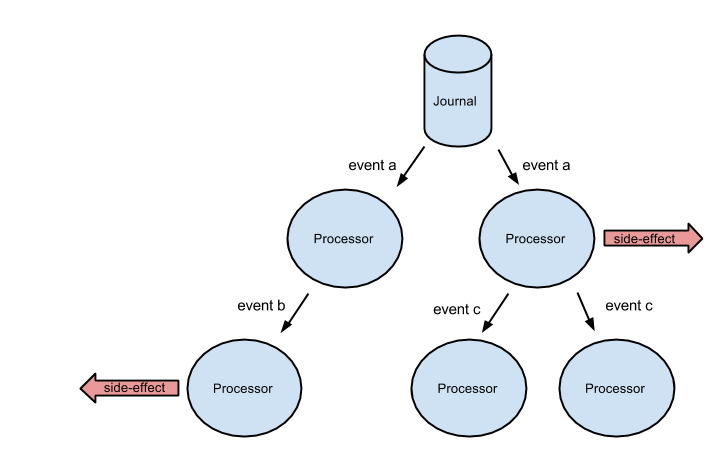
\includegraphics[width=1.0\textwidth]{img/tree.png}}
    \caption{A tree of stream processors}
    \label{fig:tree}
  \end{center}
\end{figure}

A stream processor receives events coming from its parent node. Upon the reception of an event, it can do one or several of these
actions (see Figure \ref{fig:streamprocessor}):
\begin{itemize}
  \item Creation of a sub-stream: the stream processor can transform a received event to a stream (several events), creating a sub-stream
  inside the global stream. The sub-stream must be inserted in-place in the stream: the whole sub-stream should be
  send in-order to the node's children before processing the next incoming event. For example, in Figure \ref{fig:substream},
  the processing of an input event 1 produces a sub-stream of out events 1-1, 1-2 and 1-3. Even if another input event 2
  arrives, it should not be processed before the whole sub-stream 1-1, 1-2 and 1-3 has been produced and sent to the processor's 
  children. This function is called \verb|process|.
  \item Side-effect with exactly-once semantics: The second action possible is to perform a side-effect upon each of the event
  of the sub-stream generated by the \verb|process| method. This side-effect can for example consist in updating a database representing
  a derived view on the data. This method, called \verb|performSideEffect|, must have an exactly-once semantic even in case of failures, so that the user
  can safely define non-idempotent side-effects.
\end{itemize}

\begin{figure}[H]
  \begin{center} 
    \makebox[\textwidth]{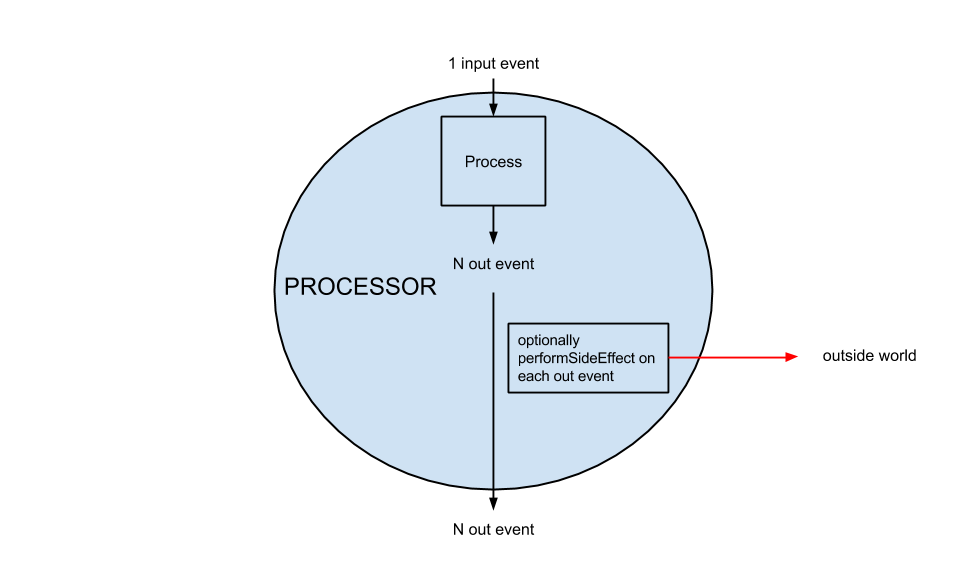
\includegraphics[width=1.0\textwidth]{img/stream_processor.png}}
    \caption{A stream processor}
    \label{fig:streamprocessor}
  \end{center}
\end{figure}

\begin{figure}[H]
  \begin{center} 
    \makebox[\textwidth]{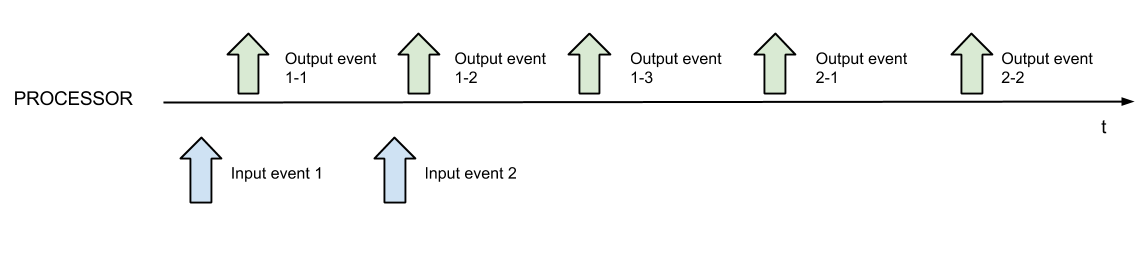
\includegraphics[width=1.0\textwidth]{img/substream.png}}
    \caption{In-order insertion of a sub-stream in a stream}
    \label{fig:substream}
  \end{center}
\end{figure}

Another important functional requirement for processors is that the \verb|process| and \verb|performSideEffect| methods can ensure the
sequentiality of asynchronous non-blocking operations (for example, a side-effect or a processing can be done via an asynchronous call to a 
database, but despite the asynchronous nature of the call the processor must wait that the asynchronous call has returned
before processing the next event). Even sub-stream production can be asynchronous, meaning that the production of a sub-stream
can be a composition of asynchronous operations (like pulling from a database with an asynchronous non-blocking driver).

Last but not least, the platform must ensure no message loss or duplication even in case of a temporary failure of a processor. This means that a processor
that had a transient failure must be able to \textit{replay} the stream from where it was before its crash.

\section{Non-functional requirements}

This section details the following non-functional requirements:
\begin{itemize}
  \item Easy scale up and scale out with a share-nothing architecture.
  \item Decoupled processors that can consume the stream with heterogeneous processing speeds without affecting each other.
  \item Optimized resource consumption in the whole system with non-blocking IO.
  \item All the previous non-functional requirements should ensure a soft real-time property (as defined in the introduction). In a few words, for a realistic event push rate as in the business use case application, the end-to-end event processing latency should be measured in seconds (not minutes or hours).
\end{itemize}

\subsection{Data Integration}

The Data Integration part must be able to scale up easily as one of the goals of the platform is to potentially handle high push rates of events. Scale up means that the puller should automatically make the best possible use of all cores available on a machine in order to parallelize the various pulls. The different parts of the puller should also be easily distributable in case of the load if too big for one machine to handle. 

To prevent software and/or hardware faults that can happen in every kind of IT systems, the puller should also be fault-tolerant, i.e if a component experiences a transient failure, the system should ensure that no event is duplicated or lost.

Moreover, the nature of the puller implies that it will spend the majority of its time doing IO to query different data sources.
Those IOs can have various durations depending on the size of the data to pull, the latency and bandwidth of the data sources, etc.
We want to optimize the use of resource (CPU, RAM) despite the fact that the platform is very IO-oriented. This enables to maximize the event push rate that a given machine can handle, and therefore minimize the cost of the infrastructure once the platform is in production. Chapter \ref{chap:study} will show how asynchronous non-blocking IO meets these expectations. 

Another non-functional requirement is to have clean and composable code source despite its asynchronous nature. Asynchronous
code can indeed lead to maintenance nightmare if the wrong abstractions are used. Chapter \ref{chap:study} will
show that the use of functional programming solves these problems.

\subsection{Journal and Stream Processing}

The Journal and Stream Processing part requires complex non-functional requirements in order to optimize resource consumption and maximize performance.

A common problem with stream processing is to manage the flow rate. A producer can indeed produce events at a rate superior to
the processing rate of a consumer. This problem is even more important when there is a tree-like structure of stream processors instead of a linear structure. Indeed, the platform should handle the fact that even if sibling processors in the tree have different processing speeds, they do not block each other based on the slowest sibling. In other words, sibling processors should be totally decoupled so that when a new event is sent from a parent to its children, the parent does not have to wait that its slowest
children has finished to process the event in order to send the next event to them. This property guarantees that a long processing will not slow down other parallel slow processing (so that an event stream that goes only through fast processors can keep a low latency). This problem should be handled while minimizing RAM consumption in order to make the best use of the resources in the system so that a given resource configuration can handle a higher push rate of events.

Stream processors should also be easily distributable in order to deal with event flows that are too big for one machine to handle.



\chapter{Study of functional programming abstractions for concurrency and asynchronicity}

The architecture of the platform is heavily based on functional programming concepts to handle concurrency and
asynchronicity in an effective and composable way. The following section describes and compares these abstractions.


\section{Monadic Futures}

\subsection{The problems of blocking IO with threads}

To handle concurrency and IO, traditional languages use native threads and blocking IO. A thread is a unit of execution that is has its own stack
on the underlining OS, and concurrency is achieved by switching threads on the machine cores. For example, with the blocking IO model,
a thread that is waiting for IO is preempted by the OS. Traditionally threads has a high resource cost, both fixed cost (the default stack size for a thread is 
1 MB on a 64 bit JVM), high context switching cost and high creation time. In case of Web-oriented application, a new thread is generally spawn for each new client,
and if the Web application needs to call several backend services (that is usually the case in modern Service Oriented Architecture), 
this thread will be blocked, doing nothing but using stack space and causing context switching.
Such a model has been proved to be inefficient for a large number of concurrent clients for Web applications that calls various backend services
and/or perform stream-oriented connections as highlighted by James Roper \footfullcite{bib:asyncio}. This is ever more
important when backend services can occasionally be slow / fail. In case of a blocking IO model, clients' threads that requests
this failed service will wait for this service (before a timeout), causing a very high number of threads in the server. As James Roper
stated, this high number of threads prevents the other requests (calling another non-failed service) to be performed efficiently,
because the server spends a lots of its time doing context switching between blocked threads that are doing nothing. This is ever worst if
you have a maximum number of threads allowed in the server (that is usually the case in cloud platforms): new clients can not connect at all
to your server because there is no thread to allow to them. Non-blocking IO servers are also known as evented servers.
Mark McGranaghan highlights this in his article about Threaded vs Evented Servers \footfullcite{bib:threadevent}. If we define \verb|c| the CPU time
that each request takes and \verb|w| the total time of the request including waiting time calling external services, an evented server
performs way better than a threaded server when the ratio \verb|w/c| is high (so when most time of a request is spent waiting for
external services).

\subsection{The problems of asynchronous non-blocking IO with callbacks}
In order to avoid the problems caused by blocking IO, one can use a non-blocking IO model: when a thread is doing an IO operation, it doesn't wait
until the IO is finished but rather provide a mechanism to notify the caller when the IO is finished. Meanwhile, the thread can be used for other tasks, like
serving other web clients. 

The problem is that this kind of asynchronous non-blocking programming can easily lead to hard code maintenance if no proper abstraction is used. The common way
of many languages to deal with asynchronicity is to provide a callback mechanism (Javascript may be the language that uses them the most). A callback is
way to perform an asynchronous operation by providing a function as a parameter of the function that do the asynchronous operation. The parameter function
will be \textit{call back} when the asynchronous operation is finished. An example of a GET HTTP request to a web service in Javascript is shown in Listing 
\ref{lst:jscb}.

\begin{listing}[h]
\begin{minted}[fontsize=\codesize, frame=lines, framesep=2mm]{javascript}
performHttpGet("http://www.example.com", function(error, response) {
  if (!error) {
    console.log("Response status: " + response.status)
  }
});
\end{minted}
\caption{A callback in Javascript}
\label{lst:jscb}
\end{listing}

Here \verb|function(error, response) {...}| is the user-defined function that is call back when the asynchronous GET request
returned. We see that callbacks are only about side-effects: no value is returned by the \verb|performHttpGet| function.
This causes a serious lack of composability, popularly known as "callback hell". Listing \ref{lst:jspd} shows how to perform several asynchronous operations
sequentially.

\begin{listing}[h]
\begin{minted}[fontsize=\codesize, frame=lines, framesep=2mm]{javascript}
action1(function(error, response1) {
  if (!error) {
    action2(function(error, response2) {
      if (!error) {
        action3(function(error, response3) {
          if (!error) {
            action4(function(error, response4) {
              // do a side-effect with response4       
            });
          }
        });
      }
    });
  }
});
\end{minted}
\caption{The "pyramid of doom" in Javascript}
\label{lst:jspd}
\end{listing}

Such call is called "pyramid of doom" because the code invariably shifts to the right, and the intermediate steps can not be reused to compose
them later with other operations. 

Moreover, doing concurrent operations with the callback model is not easy also. We want here to perform 2 asynchronous operations in parallel,
and do something with the result (composed of the result of the 2 operations). Listing \ref{lst:jsparr} shows how to do such in standard Javascript.

\begin{listing}[h]
\begin{minted}[fontsize=\codesize, frame=lines, framesep=2mm]{javascript}
  var results = [];

  function doSomethingWithResults(results) {
    // final callback
  }

  action1(function(error, response) {
      results.push(response);
      if (results.length == 2) {
        doSomethingWithResults(results)
      }
    }
  });

  action2(function(error, response) {
    results.push(response);
    if (results.length == 2) {
      doSomethingWithResults(results)
    }
  });
\end{minted}
\caption{Performing two asynchronous operations concurrently in Javascript}
\label{lst:jsparr}
\end{listing}

The fact that the callback model is based on a closures that performs side-effect prevents easy composability. What I mean by composabilty
is the fact of defining independently various asynchronous operations, and then compose them (sequentially, in parallel) to obtain a composed result
of these actions. Moreover, error handling must be done manually for each asynchronous operation. Monadic futures are an abstraction coming from
functional programming that solves these problems.


\subsection{Monadic futures for composable asynchronous non-blocking programming}

A Future is a monadic abstraction that stands for a value that may be available in the future. Using Scala's notation, a future is a type that is 
parametrized by the type of the value that will eventually be available. For example, \verb|Future[Int]| is a type that represents an eventual integer.
With futures, asynchronous functions return a \verb|Future[ResponseType]| instead of taking a callback function as a parameter. Listing \ref{lst:futures}
shows simple future creations.

\begin{listing}[h]
\begin{minted}[fontsize=\codesize, frame=lines, framesep=2mm]{scala}
val futureResponse: Future[HttpResponse] = performHttpGet("http://www.example.com")
val futureComputation: Future[Int] = future {
  // do long computation
}
\end{minted}
\caption{Futures in Scala}
\label{lst:futures}
\end{listing}

We see in Listing \ref{lst:futures} that futures can be used for non-blocking IO, but also as an abstraction for concurrency. In the example, the main thread
executing the code does not block on both methods. The "long computation" will be done in another thread as it is encapsulated by a \verb|future {}|.

Behind the scene, futures are multiplexed into a thread pool named a ExecutionContext in Scala. ExecutionContexts can be passed to methods that returned a future.
This allows to decouple the \textit{concurrency semantic} (which tasks should be run concurrently) from the \textit{concurrency implementation} (an ExecutionContext
can for example limit the number of threads it can use, etc.). Twitter's engineer and researcher Marius Eriksen highlights this idea in his 
"Your Server as a Function" paper \footfullcite{bib:serverfunc} where he states that futures are a declarative data-oriented way of doing asynchronous programming.

Moreover, as Marius Eriksen highlights in his article "Future aren't ersatz threads" \footfullcite{bib:futurenotthreads}, Futures "model the real world truthfully": 
a Future[T] can either result in a success with a value of type T, or with an error (Exception), which is inherently the case with IO operations.
\\

The term \textit{monadic} comes from Monads, a key abstraction in typed functional programming coming from the Haskell world. Thoroughly defining what a monad
is out of the scope of this thesis, but in a few words a monad is a type that encapsulates another type in order to perform operations on it. Some operations
are mandatory to define a monad. Listing \ref{lst:monad} define the trait in Scala to define a monad, coming from the book Functional Programming in Scala
\footfullcite{bib:fpscala}. 

\begin{listing}[h]
\begin{minted}[fontsize=\codesize, frame=lines, framesep=2mm]{scala}
trait Monad[F[_]] extends Functor[F] {
  def unit[A](a: => A): F[A]
  def flatMap[A,B](ma: F[A])(f: A => F[B]): F[B]

  def map[A,B](ma: F[A])(f: A => B): F[B] = flatMap(ma)(a => unit(f(a)))
}
\end{minted}
\caption{The Monad trait in Scala}
\label{lst:monad}
\end{listing}

\verb|unit| allows to construct a monad that encapsulate a value of type A (equivalent to \verb|future {}|), \verb|map| allows to apply a function to 
the encapsulated value, and \verb|flatMap| allows to apply a function to the encapsulated value that returns itself a monad.
\\

A Future is a monadic type, meaning that it extends the monad trait and implement the \verb|unit| and \verb|flatMap| methods.
These methods (and many more) allows powerful compositions between different Futures instances. A Future is also an immutable
data structure with all the functional programming benefits related to it (safe sharing between threads, ease of reasoning with referentially transparent code, etc).

For example, \verb|map| allows to transform the result of an asynchronous operation. \verb|flatMap| allows sequential and 
parallel composition. \textit{flat} comes from \textit{flatten} because flatMap can transform a Future[Future[T]] to a Future[T].
Listing \ref{lst:futcompo} illustrates these composition.

\begin{listing}[h]
\begin{minted}[fontsize=\codesize, frame=lines, framesep=2mm]{scala}
/*
 * Sequential composition of asynchronous operations returning Integers
 */
val future1: Future[Int] = action1()
val future2: Future[Int] = future1 flatMap (result1 => action2(result1))
val future4: Future[String] = future2
  .flatMap(result2 => action3(result2))
  .flatMap(result3 => action4(result3))
  .map(result4 => "This is result4: " + result4)

/*
 * Concurrent composition
 */
val future1: Future[Int] = action1()
val future2: Future[Int] = action2()
val future1And2: Future[(Int, Int)] = future1 zip future2
// "zip" is another monad-ish operation for composition 
\end{minted}
\caption{Future composition in Scala}
\label{lst:futcompo}
\end{listing}

We see in Listing \ref{lst:futcompo} that we avoid the "pyramid of doom" effect for sequential composition, and that concurrent composition is very simple
compared to callback-based programming. Moreover, monad operations allows automatic error propagation. In the sequential composition example,
if for instance action2 failed, the action3 and action4 will not be executed, and futureResult4 will be a failed future with the Exception
that action2 throwed. For more examples, LinkedIn's engineer Yevgeniy Brikman highlights the composability of Futures in his article named
"Play Framework: async I/O without the thread pool and callback hell" \footfullcite{bib:playasyncio}.
\\

In summary, a monadic future is a immutable abstraction for concurrency and asynchronism that allows easy reasoning and composition.
However, a future only model the fact that \textit{one} value will be available in the future. Hence, it is not directly applicable
to model asynchronous non-blocking \textit{streams}.

\subsection{Promises}
\label{sec:promises}
A promise is an abstraction that can be seen as a Writable Future. One can create a Promise, and get a Future from it. Then, when one call the method promise.success(value),
the related Future is fulfilled asynchronously with this value. Listing \ref{lst:promiseexample} illustrates the use of Promises. 

\begin{listing}[h]
\begin{minted}[fontsize=\codesize, frame=lines, framesep=2mm]{scala}
val promise1 = promise[Int]
val future1 = promise1.future

val future2 = future1 map (value => value + 1) // future2 will eventually contain the value 2

// ...

promise1.success(1) // triggering future1 with the value 1
\end{minted}
\caption{Promises in Scala}
\label{lst:promiseexample}
\end{listing}

Promises can for example be used to let communicate a consumer and a producer as we will see in the Stream Processing architecture and implementation chapter.

\section{Iteratees}
\label{sec:iteratees}

To model streams that can be produced in an asynchronous non-blocking way, the Iteratee abstraction can be used. An iteratee is an immutable data structure
that allows incremental, safe, non-blocking and composable stream processing. One key feature of Iteratee is \textit{back-pressure} that will be described later on.
The Iteratee way of processing stream involves three abstractions: Enumerators, Enumeratees and Iteratees. The Iteratee library from Play Framework 
\footfullcite{bib:playiteratees} is used for the examples.
\\

An Iteratee is a stream consumer and is represented by the type \verb|Iteratee[E, A]|. An iteratee receive chunks of type \verb|E| 
in order to produce a result of type \verb|A|. The main method of an iteratee is a fold method that passes around its current state and the
next chunk to process.
Listing \ref{lst:iterateecount} shows how to define an iteratee that sums the number of characters it receives.

\begin{listing}[h]
\begin{minted}[fontsize=\codesize, frame=lines, framesep=2mm]{scala}
val chunkCounter: Iteratee[String, Int] = Iteratee.fold { (chunk, nbBytesReceived) =>
  nbBytesReceived + chunk.length
}
\end{minted}
\caption{A counter Iteratee}
\label{lst:iterateecount}
\end{listing}

An Enumerator is a stream producer of type \verb|Enumerator[E]|. Listing \ref{lst:enumerators} shows how to create an enumerator that streams a collection.

\begin{listing}[h]
\begin{minted}[fontsize=\codesize, frame=lines, framesep=2mm]{scala}
val producer: Enumerator[String] = Enumerator.enumerate(List("foo", "bar", "foobar"))
\end{minted}
\caption{A simple enumerator}
\label{lst:enumerators}
\end{listing}

An Enumeratee is a stream transformer of type \verb|Enumeratee[E, F]| transforming chunks of type E to chunks of type F.
Listing \ref{lst:enumeratees} shows several enumeratee examples.

\begin{listing}[h]
\begin{minted}[fontsize=\codesize, frame=lines, framesep=2mm]{scala}
val filter = Enumeratee.filter[String](chunk => chunk != "bar")
val mapper = Enumeratee.map[String](chunk => chunk + "!")
\end{minted}
\caption{Map and filter enumeratees}
\label{lst:enumeratees}
\end{listing}

An interesting properties of Iteratees/Enumerators/Enumeratees is that they can be easily composed. Listing \ref{lst:iterateecompo}) shows how to
run the data flow. As all is asynchronous, a Future of the result is returned. 

\begin{listing}[h]
\begin{minted}[fontsize=\codesize, frame=lines, framesep=2mm]{scala}
// An composed enumeratee that will perform filter and map to the stream
val filterAndMapper: Enumeratee[String, String] =  filter compose mapper

// A composed enumerator which produces chunk that will be filtered and mapped
val modifiedProducer: Enumerator[String] = producer through filterAndMapper

// Please note that all the operations were lazy for now.
// Now we run the enumerator into the iteratee in order to process the flow
val futureResult: Future[Int] = modifiedProducer run chunkCounter
// the future result will be "foo!".length + "foobar!".length == 11
\end{minted}
\caption{Stream composition}
\label{lst:iterateecompo}
\end{listing}

During the stream processing, either the Enumerator can choose to end the stream (sending an EOF) or the Iteratee can choose that it has processed enough
chunk to compute its final value and stop the stream processing by returning a Done state to the Enumerator.
\\

A very interesting feature is when we have to compose asynchronous operations in order. Iteratees allows to define
producer, transformer and consumer that return Futures of their operations. Moreover, Play Framework's Iteratee library
provides helpers that allows for example to fetch an HTTP stream in a non-blocking way through an Enumerator.
Listing \ref{lst:asynciteratee} shows how to get a Http stream (for example a stream of tweets), call an external web service to process
the chunks, and insert the processed chunks in a database with the position of this chunk in the stream. 
The Iteratee design ensures that chunks will be process in the order of the producer, even with asynchronous
operations during the processing flow.

\begin{listing}[h]
\begin{minted}[fontsize=\codesize, frame=lines, framesep=2mm]{scala}
val asyncProducer: Enumeratee[String] = getHttpStream("http://example.com/stream")

val asyncTransformer: Enumeratee[String] = Enumeratee.mapM { Chunk => 
  val futureProcessedChunk: Future[String] = callWebService(Chunk)
  futureProcessedChunk
}

val asyncDatabaseSink = Iteratee.foldM[String, Int](0) { (processedChunk, n) =>
  val futureInserted = database.insert((processedChunk, n))
  futureInserted map (_ => n + 1)
}

// Starting the processing
asyncProducer through asyncTransformer run asyncDatabaseSink
\end{minted}
\caption{Asynchronous non-blocking stream processing}
\label{lst:asynciteratee}
\end{listing}

In the example of Listing \ref{lst:asynciteratee}, chunks are guaranteed to be in-order when they are inserted in the database. The \verb|M| after
the \verb|map| and \verb|fold| methods stands for Monad, that is in our case a Future.

Under the hood, an Enumerator is a kind of fold method that push chunks in a Iteratee. An Iterate can be in \verb|Cont| state meaning that it wants to consume more 
chunks from an enumerator, in \verb|Done| state
meaning that it does not want more input to compute its result value, or in \verb|Error| state. For each chunk, the Iteratee returns to the Enumerator
a Future of its state. When this future is redeemed, it means that the Iteratee has finished processing the current chunk, so the enumerator can 
push the next chunk into it (which can be also done by returning a Future of the chunk). Figure \ref{fig:itenum} illustrates this mechanism.

\begin{figure}[h]
  \begin{center} 
    \makebox[\textwidth]{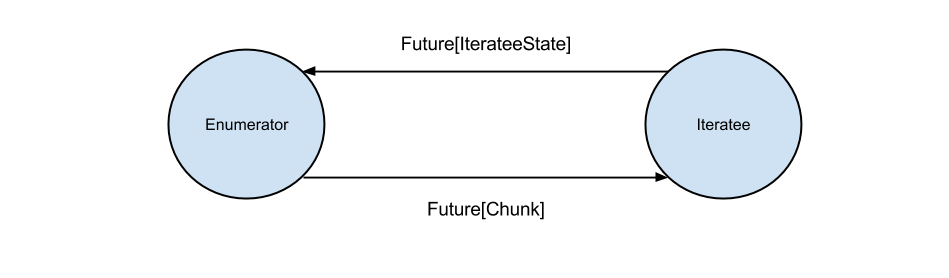
\includegraphics[width=1.0\textwidth]{img/itenum.png}}
    \caption{Back-pressure mechanism with Enumerator and Iteratee using Futures}
    \label{fig:itenum}
  \end{center}
\end{figure}

Thus we have asynchronous production and consumption with the consumer that "tells" (via its future state) to the producer that it is ready to 
consume more chunks (or not). This mechanism in known as \verb|back-pressure| and allows the consumer to slow down the producer rate depending on its 
own processing speed. 

With back-pressure, we can differentiate two kinds of producers: \textit{cold} sources and \textit{hot} sources. Cold sources are sources that
produces chunks from a static durable collection, meaning that the consumer can process the stream at his own speed without the risk of losing events.
On the contrary, \textit{hot} sources are for example events coming from a network connection. If the consumer is not ready to consume the next chunk,
a choice has to be done (drop the event, buffer it, ...). These problems will be dealt with more specifically further in the report.
\\

Futures and Iteratees compositions allows to model the asynchronous processing of both a single value and a stream of values, but 
they are not abstractions to built your entire program on (they are parts of your program).
The Actor model is an abstraction to model your entire application to easily handle concurrency, distribution and fault-tolerance, and can use Futures and Iteratees.

\section{Actor model}

First of all, it should be noted the Actor model is not a purely functional model as it use some side-effects. It is generally said that it sits between functional and
imperative. Nevertheless, we will study it in this part as it integrates very well with functional code and is part of Scala's way of handling concurrency.
The examples use the Akka framework \footfullcite{bib:akka} that provides actor systems for the JVM in Scala.
\\

\subsection{The actor model in Akka}

In imperative languages, synchronization of different concurrent operations is usually done by using locks (including synchronization blocks in Java). 
However, locks is a very low-level primitive that can easily lead to problems like dead-lock, data inconsistency if not enough locks, 
slow performance if too many locks. Moreover, IO is generally done explicitly via sockets.

An actor system is a higher level abstraction to deal with concurrency and synchronization, and abstracts away sockets by providing a location transparent model
via message passing. It enables simple fault-tolerance and distribution.
\\

An actor is a lightweight concurrent entity. Basically, an actor receives messages from other actors and send messages to other actors. Upon the reception of 
a message, it can modify its internal state (actors can be stateful), send messages to other actors, and change its message handling behavior of the next messages.
Each actor has one mailbox that corresponds to a FIFO queue of incoming messages.
It is guaranteed that message processing is sequential inside a same actor, i.e one should not have to worry about concurrency problems inside an actor. Listing
\ref{lst:actorexample} shows how to define a simple Actor that counts the number of messages it receives. Messages can sent to him concurrently without worrying
about synchronization problems.

\begin{listing}[h]
\begin{minted}[fontsize=\codesize, frame=lines, framesep=2mm]{scala}
case object Message

class Counter extends Actor {
  var counter = 0

  def receive = {
    case Message => 
      counter = counter + 1
  }
}

val system = ActorSystem("MySystem")
val counter = system.actorOf(Props[Counter], name = "counter")

// Sending concurrently 100 messages to the actor 
// (the send operation "!" do not block or wait for an ack)
(1 to 100).par foreach (_ => counter ! Message)
\end{minted}
\caption{A counter actor}
\label{lst:actorexample}
\end{listing}

Another important part of the actor model of Akka is the Tree-like hierarchical organization between actors, called Supervision.
A parent that create child actors is responsible for them, meaning that it should handle their possible failures (by stopping them,
restarting them, etc).
\\

Last but not least, the fact that actors communicates only via message passing (share-nothing architecture) allows location transparency, which
enables easy distribution. In Akka, the fact that one or several actors are located on different machines is written in a configuration file, meaning that
one can write the exact same code for a program that execute locally or in a distributed fashion.

Under the hood, a Scheduler is in charge of multiplexing actors into threads, like the ExecutionContext multiplexes Futures into threads.

\subsection{Mixing Actors with Futures}
\label{sec:mixingactorfuture}

Akka's actors can be used with library that use Futures. However, one should pay attention to the mix between SchedulerContext 
and futures' ExeceutionContext. Akka ensures that all message processing are sequential (so that one does not have to worry about concurrency problems inside
an actor), but if the result of a future tries to modify the internal state of an actor, Akka can not ensure the sequentiality as it only control the SchedulerContext
that is used to process incoming messages. To avoid this, one must use the \textit{pipeTo} pattern that transform the result a Future in a message sent to the actor.
Listing \ref{lst:akkasafeunsafe} illustrates this mechanism.

\begin{listing}[h]
\begin{minted}[fontsize=\codesize, frame=lines, framesep=2mm]{scala}
case class Message(data: String)
case class Result(result: String)

// An actor that receive a Message, call an async method to process it,
// store the result of the processing
class ProcessActor extends Actor {
  var storeResults = Seq.empty[String]

  def receive = {
    case Message(data: String) => 
      val futureResult = process(data)
      futureResult map { result =>
        Result(result)
      } pipeTo self

    case Result(result: String) =>
      storeResults = storeResults :+ result
  }
}

// Below is an example that is concurrently unsafe because the future 
// modify the internal state of the actor
class UnsafeActor extends Actor {
  var storeResults = Seq.empty[String]

  def receive = {
    case Message(data: String) => 
      val futureResult = process(data)
      futureResult foreach { result =>
        storeResults = storeResults :+ result
      }
  }
}
\end{minted}
\caption{Mixing Futures with Actors}
\label{lst:akkasafeunsafe}
\end{listing}

The following chapter describes the architecture and implementation of the platform that makes heavy use of the functional programming abstractions which have been 
presented in this chapter.



\chapter{Architecture and implementation of the Data Integration part}

As stated in the Requirements chapter, the Data Integration part must incrementally pull various REST APIs (data sources) in parallel. For each resource type in
in each data source, it must create an event flow. This event flow run through several data cleaning and data transformation steps that can
be asynchronous. Despite the asynchronous nature, it should ensure that the event flow remains in-order. In the end, event flows are pushed
into the Journal.

\section{Architecture}

\subsection{Puller actor system}

In order to pull periodic incremental pull of data sources, an Akka Actor system is defined. 

First, the system needs for each data source to receive a "top" message corresponding to the fact that a certain data source must be queried. We will use for this
Akka Quartz \footfullcite{bib:akkaquartz}, a cron-style scheduler that allows to define periodic sending of certain types of messages. An usual pull rate for a data source
is every 5 seconds, in order to create a near-realtime stream.
\\

These top messages will be received by a singleton actor named \verb|JobScheduler|. The purpose of the JobScheduler is to launch a child actor for each job (a job
corresponds to an incremental pull from a certain data source). Once the child actor has finished the incremental pull, it kills itself. Figure \ref{fig:archi_actor_dataintegration} illustrates this architecture.

\begin{figure}[h]
  \begin{center} 
    \makebox[\textwidth]{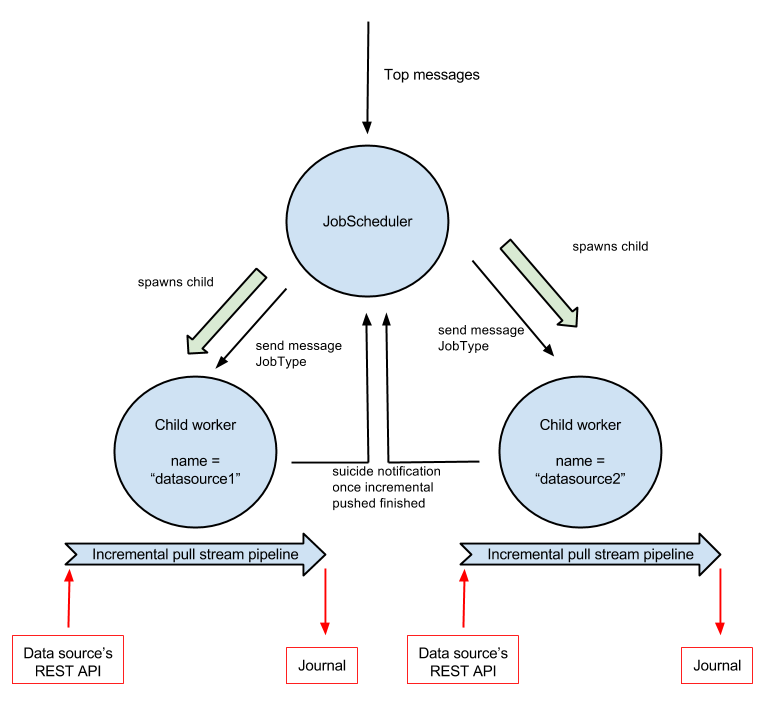
\includegraphics[width=1.0\textwidth]{img/archi_actor_dataintegration.png}}
    \caption{Puller actor system}
    \label{fig:archi_actor_dataintegration}
  \end{center}
\end{figure}

The JobScheduler must handle the fact that the job message rate for a data source can be faster than the incremental pull
of this data source (for example if the data source has produced a lot of new data since the last pull, or if it experiences some network problems). If a pull is still running when 
a new job message arrives for a data source, the JobScheduler should ignore the new pull message to avoid doing two or more pull in parallel of the same data source and risking a wrong
order of events. The JobScheduler can do this by assigning the name of the data source when it spawns a new worker child. Then, when a new job message comes in, it checks if it has a child of this name, and only if such child doesn't exist it spawns a new child.

The actor model also allows to deal with errors. In our case, we just want to ignore the failure of a child worker. The next top message for this data source will automatically
launch a new child worker for this data source. Thus, the JobScheduler actor will have a special Supervision Strategy that ignore the failure of its children.


\subsection{Incremental pull jobs}

When it is launched, each job must do an incremental pull on a particular data source via its REST API. For each the data source that the platform must integrate, there exists
a GET method that allows to get all the resource ids that were updated in a descendant order. The GET response is paginated, meaning that ids are coming 50 by 50 for example (the 
API caller has to make several call until it has all the ids it wants). 

A pull job has to pull the event ids that were updated after the last incremental pull. To do this, we define a stream where the producer makes one or several call to the
paginated REST API to produce a stream of JSON containing the ids of the resources updated. The producer must stop pulling when the date of the current update is less than the last
update event processed during the previous job. In order to persist for each job the date of the last event processed, we use a MongoDB database with a collection that stores a 
document with all the last event processed of each data source.

Moreover, for each resource, we are only interested in keeping the last update. Indeed, the REST API only gives us the type of update with the id of the resource, so if we pull (in desc order) a delete event before an update event, we want only to retain the delete event.

Then, the stream of events should be re-sorted in ascendant order, then for each event we must query the REST API to transform the resource id in the resource itself, then we must clean the resulting JSON to transform it to a known data model, then create an Journal event to insert in the Journal, and finally update MongoDB with the date of the last event.
Figure \ref{fig:datintflow} illustrates this pipeline in a simple schema. 

\begin{figure}[h]
  \begin{center} 
    \makebox[\textwidth]{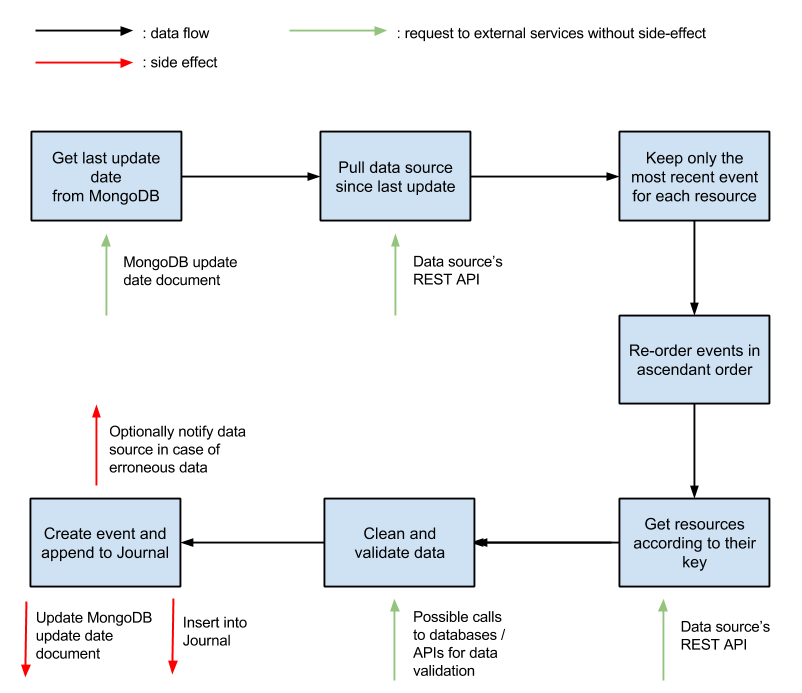
\includegraphics[width=1.0\textwidth]{img/datintflow.png}}
    \caption{Incremental pull stream pipeline}
    \label{fig:datintflow}
  \end{center}
\end{figure}

We see in Figure \ref{fig:datintflow} that the data stream pipeline must asynchronously process (calling external services) events while keeping ordering of messages, so Iteratees and Futures will be used to meet these requirements.
Moreover, an effort is made to isolate side-effects at the end of the stream pipeline in order to enable easy reuse of intermediate blocks. Isolation of side effects for better code
reuse and reasoning is one of the core principles of functional programming.
\\

Such an architecture allows transparent concurrency and parallelism up to the number of cores. Each child actor is executed concurrently, and the asynchronous stream processing
is using Iteratees that use Futures to allow transparent concurrency. If we give to the Iteratees/Futures the SchedulerContext as ExecutionContext, we share threads between actors
and futures, which will create the best possible use of cores in the machine (the total number of threads roughly equals to the number of cores).

Moreover, in case the system needs to scale out, the Actor model also allows easy distribution. In this architecture, the JobScheduler can transparently spawns some worker 
children in other machines. The implementation part will detail this part more thoroughly.


\section{Implementation}

\subsection{Puller actor system}

The Akka framework is used to implement the puller actor system in Scala. The JobScheduler is the main/master actor that receives top messages related to a data source and a special
kind or resource, and spawns a new worker child to accomplish this task only if it has not already a child doing this particular task. Listing \ref{lst:akkajobscheduler} shows the
code of the JobScheduler actor.

\begin{listing}[h]
\begin{minted}[fontsize=\codesize, frame=lines, framesep=2mm]{scala}
class JobScheduler extends Actor {
  private val logger = LazyLogger.apply("services.JobScheduler")

  override val supervisorStrategy = stoppingStrategy
  
  def receive = {
    case jobType: JobMessage =>
      // ensure sequentiality of the iterations of a same job
      val isRunning = context.child(jobType.toString) map (_ => true) getOrElse false
      if (!isRunning) {
        logger.info("Launching child...")
        val worker = context.actorOf(Props[JobWorker], name = jobType.toString)
        worker ! jobType
      } else {
        logger.warn("Job " + jobType + " ignored because the previous iteration 
                                                  of the job is still running.")
      }
  }
}
\end{minted}
\caption{JobScheduler actor}
\label{lst:akkajobscheduler}
\end{listing}

The \verb|supervisorStrategy| is set to \verb|stoppingStrategy| in order to ignore possible failures of children. Listing \ref{lst:akkajobworker} shows the worker actor code.

\begin{listing}[h]
\begin{minted}[fontsize=\codesize, frame=lines, framesep=2mm]{scala}
class JobWorker extends Actor {
  private val logger = LazyLogger.apply("services.JobRunner")
  
  type Job = () => Future[Int]
  case object JobFinished
  
  def receive = {
    case jobType: JobMessage =>
      val job = getLazyJob(jobType)
      job() map { result =>
        logger.info("Finished " + jobType + " job successfully: " + result)
        JobFinished
      } recover { case error: Throwable =>
        logger.error("Finished " + jobType + s" job with error: 
                                  $error\n${error.getStackTraceString}")
        JobFinished
      } pipeTo self
    
    case JobFinished => context.stop(self)
  }

  def getLazyJob: JobMessage => Job = {
    case DataSource1ResourceType1 => DataSource1ResourceType1.job

    case DataSource1ResourceType2 => DataSource1ResourceType2.job

    case DataSource2ResourceType1 => DataSource2ResourceType1.job

    ...
  }
  
}
\end{minted}
\caption{JobWorker actor}
\label{lst:akkajobworker}
\end{listing}

The type \verb|Job| is the type that must be implemented for an incremental pull stream job. \verb|() => Future[_]| means that the pull job must be a function that take no
parameter and return a Future of Int. This Future of Int will be fulfilled when the pull job is finished with the number of Journal events that were created during this iteration
of the incremental pull job. Upon the completion of the future, we map it to a \verb|JobFinished| message that we pipe to \verb|self| (the current actor). Upon the reception
of this message, it knows that the job is finished, and so it kills itself (his parent actor JobScheduler will be automatically notified by its death). Please note that
\verb|context| is part of the actor internal state, so it is not safe to access it into the Future as we saw in section \ref{sec:mixingactorfuture}. That's why we pipe the future to
a message that will be sent to the actor.
\\

The module Akka Quartz allows to define in a configuration file the periodicity of the top messages that will be sent to the JobScheduler actor. See the configuration 
file shown in Listing \ref{lst:configquartz} for an example.

\begin{listing}[h]
\begin{minted}[fontsize=\codesize, frame=lines, framesep=2mm]{scala}
akka {
  quartz {
    schedules {

      DataSource1ResourceType1 {
        description = "Fire DataSource1ResourceType1 every 5 seconds"
        expression  = "*/5 * * ? * *"
      }

      DataSource1ResourceType2 {
        description = "Fire DataSource1ResourceType2 every 2 seconds"
        expression  = "*/2 * * ? * *"
      }

      DataSource2ResourceType1 {
        description = "Fire DataSource2ResourceType1 every 5 seconds"
        expression  = "*/5 * * ? * *"
      }
        
    }
  }
}
\end{minted}
\caption{Cron-style configuration to schedule jobs}
\label{lst:configquartz}
\end{listing}

\subsection{Example of a incremental pull job}

In this section we will describe the implementation of an incremental pull jobs. We take for example a job that pull every 5 seconds the resources of a certain type, called Credit Notes, that has been created, updated or deleted in a SaaS financial software (called FinancialSoftware for this report).
\\

Iteratees and Futures are used to model asynchronous non-blocking stream processing. As we will see, the composabilty of Iteratees allows a very clear modularization of the 
different processing components. 

\subsubsection{Enumerator of Events coming from FinancialSoftware}

The first step is to create an enumerator (a producer) that pull events that happened to a certain resource type since the last pull. The REST API
of FinancialSoftware is paginated by 50, meaning that a GET request on the last events only give the 50 events, and a link the next "page" containing the next 50 events.
The enumerator has to pull the REST API until it detects that the current event has a date inferior to the last update date.
\\

We have to use an enumerator that repeatedly fetch pages from the FinancialSoftware REST API until it has streamed all the events since a date named \verb|since|, and return
a stream of \verb|FinancialSoftwareEvent| containing each the id of a resource of certain type with its related event (create, update or delete) and its date. 
Listing \ref{lst:enumfetchsellsy} shows the code of such enumerator.

\begin{listing}
\begin{minted}[fontsize=\codesize, frame=lines, framesep=2mm]{scala}
case class Page(nb: Int, totalNbPages: Int, docs: Seq[JsObject])
case class FinancialSoftwareEvent(documentId: String, updateType: String, date: DateTime)

object FinancialSoftware {
  private val dateFormat = DateTimeFormat.forPattern("yyyy-MM-dd HH:mm:ss")

  val apiUrl = "..."
  val authentificationParams = "..."

  def retrieveUpdates(resourceType: String, since: DateTime): 
      Enumerator[FinancialSoftwareEvent] = {

    def getPage(nb: Int): Future[Page] = {
      val url = apiUrl + "/" + resourceType + "?" + authentificationParams + "&page=" + nb
      WS.url(url).get map { response =>
        val json = Json.parse(response.body)
        val nbPage = (json \ "pagenum").as[Int]
        val totalNbPages = (json \ "nbpages").as[Int]
        val docs = (json \ "results").as[Seq[JsObject]]
        Page(nbPage, totalNbPages, docs)
      }
    }

    val producer: Enumerator[Seq[JsObject]] = 
      Enumerator.unfoldM[Option[Int], Seq[JsObject]](Some(1)) {
        case Some(nextPageNb) =>
          getPage(nextPageNb) map { nextPage =>
            if (nextPage.nb < nextPage.totalNbPages) {
              Some((Option(nextPage.nb + 1), nextPage.docs))
            } else {
              // last page
              Some(None, nextPage.docs)
            }
          }
        case None => Future.successful(None)
      }

    val flattenedProducer: Enumerator[JsObject] = 
      producer &> Enumeratee.mapConcat(identity)

    flattenedProducer &>
    Enumeratee.map { jsObject =>
      val id = (jsObject \ "relatedid").as[String]
      val date = (jsObject \ "date").as[DateTime]
      val eventType = (jsObject \ "type").as[String]
      FinancialSoftwareEvent(id, eventType, date)
    } &>
    Enumeratee.takeWhile { event =>
      event.date.compareTo(since) > 0
    }
  }
}
\end{minted}
\caption{Enumerator that stream the last events of a data source}
\label{lst:enumfetchsellsy}
\end{listing}

The main method to call is \verb|retrieveUpdates| that returns an Enumerator[FinancialSoftwareEvent]. The \verb|&>| operator between an enumerator and an enumeratee
is an alias for the \verb|through| composition method explained in section \ref{sec:iteratees}.

\subsubsection{Stream pipeline composition}

From this producer of \verb|FinancialSoftwareEvent|, we want to apply several operations to the stream processing pipeline as illustrated in Figure \ref{fig:datintflow}. 
First, we want to keep only the most recent event of each resource. Listing \ref{lst:keepHeadId} shows how to define such an Enumeratee. It returns a 
\verb|Map[String, FinancialSoftwareEvent]| where document id is the key and the last event (so the first in the descendant order stream) related to this document (resource)
is the value.

\begin{listing}[h]
\begin{minted}[fontsize=\codesize, frame=lines, framesep=2mm]{scala}
def groupByDocumentIdKeepingHeadEvent: 
    Enumeratee[FinancialSoftwareEvent, Map[String, FinancialSoftwareEvent]] = {

  Enumeratee.grouped(Iteratee.fold(Map.empty[String, FinancialSoftwareEvent]) { 
    (record, financialEvent) =>
      val id = financialEvent.documentId
      if (!record.contains(id))
        record + (id -> financialEvent)
      else record
  })
}
\end{minted}
\caption{Enumeratee that keeps only the most recent FinancialSoftwareEvent of each resource}
\label{lst:keepHeadId}
\end{listing}

Then, we must create an enumeratee that transform this Map in a stream of event in ascendant date order (see Listing \ref{lst:enumreorder}).

\begin{listing}[h]
\begin{minted}[fontsize=\codesize, frame=lines, framesep=2mm]{scala}
val reorder: Enumeratee[Map[String, FinancialSoftwareEvent], FinancialSoftwareEvent] = 
  Enumeratee.mapConcat { mapIdToEvent => 
    val ascendingSeqOfEvents = mapIdToEvent.toSeq.sortBy { case (id, event) => event.date }
    ascendingSeqOfEvents
  }
\end{minted}
\caption{Enumeratee that re-order events in ascendant order}
\label{lst:enumreorder}
\end{listing}

Then, we must call again the data source's REST API to transform the documentId by the document (resource) itself (see Listing \ref{lst:enumgetdoc}).
Note the use of Enumeratee.mapM that allows sequential (in-order) composition of an asynchronous operation that returns a Future (FinancialSoftware.getResource).

\begin{listing}[h]
\begin{minted}[fontsize=\codesize, frame=lines, framesep=2mm]{scala}
def getDocument(resourceType: String): 
    Enumeratee[FinancialSoftwareEvent, (JsObject, String, DateTime)] =

  Enumeratee.mapM { event =>
    val id = event.documentId
    FinancialSoftware.getResource(resourceType + "/" + id) map { response =>
      (response \ "response").as[JsObject], event.updateType, event.date)
    }
  }
\end{minted}
\caption{Enumeratee that get a resource according to its id}
\label{lst:enumgetdoc}
\end{listing}

Then, several other Enumeratees are created to clean and validate the data that will not be shown here because the code is long and very data specific.
We name this resultant enumeratee cleanAndValidate of type Enumeratee[(JsObject, String, DateTime), Command[ZEvent]], ZEvent being the type of the Journal events. 
Listing \ref{lst:zevent} shows the case class ZEvent which will be more detailed in the Journal and Stream Processing part. 

The \verb|Command| type is a functional type that allows to accumulate the side-effect to do at the end of the pipeline. For example, in the data validation part, the
detection of erroneous data may imply to send a message back to the data source (this type of side-effect is called Annotation). To enhance code re-usability and correctness according to functional programming, the Command type accumulates the different type side-effects that may be done at the end of the pipeline. The final Iteratee that do all the side-effects
is named performSideEffects. It takes a stream of Command[ZEvent], send the possible annotations to the data source, write the possible ZEvent to the Journal and update
the MongoDB collection that stores the date of the last event processed. The type is
Option[ZEvent] because sometimes if data validation fails we don't even want to write an event in the Journal. Listing \ref{lst:finaliterateedataint} illustrates the Command
type and the performSideEffects iteratee (note that for log purpose, the iteratee counts the number of events it has sent to the Journal).

\begin{listing}[h]
\begin{minted}[fontsize=\codesize, frame=lines, framesep=2mm]{scala}
case class ZEvent(
  id: PathId,
  resource: String,
  user: String,
  date: DateTime,
  name: String,
  body: JsObject)
\end{minted}
\caption{ZEvent: a Journal event}
\label{lst:zevent}
\end{listing}

\begin{listing}[h]
\begin{minted}[fontsize=\codesize, frame=lines, framesep=2mm]{scala}
case class Command[A](date: DateTime, maybeEvent: Option[A], annotations: List[Annotation]) 

def performSideEffects: Iteratee[Command[ZEvent], Int] =
  Iteratee.foldM(0) { case (nbEvents, Command(eventDate, maybeEvent, annotations)) =>
    annotations foreach { annotation =>
      annotation.annotate() // send to data source
    }
    maybeEvent match {
      case Some(event) =>
        for {
          _ <- RefJournal.write(event)
          _ <- setLastUpdate(jobKey, eventDate) // set last update date
        } yield nbEvents + 1
      case None =>
        setLastUpdate(jobKey, eventDate) map (_ => nbEvents)
    }
  }
\end{minted}
\caption{PerformSideEffects Iteratee}
\label{lst:finaliterateedataint}
\end{listing}

Thus, we have separately define data producers (enumerator), data transformers (enumeratee) and data sink (iteratee). We now just have to connect them together. Composability
and static typing allows to do so easily, safely and clearly (see Listing \ref{lst:fullpipelinedataint}). The final type of the job method is Job, the alias type for
() => Future[Int] that were defined in the Puller actor system implementation section.

\begin{listing}[h]
\begin{minted}[fontsize=\codesize, frame=lines, framesep=2mm]{scala}
object FinancialSoftware {
  def job: Job = {
    val resourceType = "exampleResource"
    val since = DateTime.now

    val futureLastEventDate = getLastUpdate(resourceType)

    val futureNbEventsInserted: Future[Int] = futureLastEventDate flatMap { lastEventDate =>
      retrieveUpdates("resourceType1", since) &>
      groupByDocumentIdKeepingHeadEvent &>
      reorder &>
      getDocument(resourceType) &>
      cleanAndValidate |>>>  // |>>> is an alias for "run"
      performSideEffects
    }
  }
}

\end{minted}
\caption{Whole stream processing pipeline from a data source to the Journal}
\label{lst:fullpipelinedataint}
\end{listing}


\subsection{Distribution}

This architecture can be easily distributed thanks to actor systems' location transparency. Actually, the above code doesn't need any changes to run it in a distributed
environment. 
For example, we want the worker children that pull DataSource1 to be executed on a remote machine different than the master machine where the JobScheduler actor runs.
We can use the Akka Remote module \footfullcite{bib:akkaremote} for this use case. It allows via a configuration file to configure the JobScheduler actor to create some
of its children in a remote machine rather than locally. The configuration file shown in Listing \ref{lst:configremotemaster} should be put in the master node and 
tells the JobScheduler to create the child actor of names DataSource1ResourceType1 and DataSource1ResourceType2 on the remote machine of address 127.0.0.1:2553.

\begin{listing}[h]
\begin{minted}[fontsize=\codesize, frame=lines, framesep=2mm]{scala}
# Akka master node
akka {
  actor {
    provider = "akka.remote.RemoteActorRefProvider"
    deployment {
      /master/SellsyCreditnotesJob {
        remote = "akka.tcp://remote@127.0.0.1:2553"
      }
    }
  }
  remote {
    enabled-transports = ["akka.remote.netty.tcp"]
    netty.tcp {
      hostname = "127.0.0.1"
      port = 2552
    }
  }
}
\end{minted}
\caption{Configuration file for master node - Akka Remoting}
\label{lst:configremotemaster}
\end{listing}

On the worker machine, an actor system of name "remote" should be launch with the configuration file shown in Listing \ref{lst:configremoteworker}. Moreover,
one should ensure that the JVM classloader on the worker machine has a JAR containing the class JobWorker.

\begin{listing}[h]
\begin{minted}[fontsize=\codesize, frame=lines, framesep=2mm]{scala}
# Akka worker node
akka {
  actor {
    provider = "akka.remote.RemoteActorRefProvider"
  }
  remote {
    enabled-transports = ["akka.remote.netty.tcp"]
    netty.tcp {
      hostname = "127.0.0.1"
      port = 2553
    }
  }
}  
\end{minted}
\caption{Configuration file for worker node - Akka Remoting}
\label{lst:configremoteworker}
\end{listing}

Thus, we transform our system to a mutli-core local system to a distributed system without having to change to code. This can be very useful for systems that first have enough
resources with one machine, but after a while needs to be put on several machines for scalability.
\\

However, one problem with the approach of Akka Remoting is that it is "end-point to end-point" oriented, meaning that the jobs for data source X or Y are statically
mapped to one machine. For elastic and adaptive scalability, it would be more interesting to give a bunch of worker machines to Akka, and it will determine itself on which machine 
it is better to launch the new child worker according to the current resource availability of the machines (CPU, RAM, ...).

This approach in currently under development in Akka and is named Akka Cluster \ref{bib:cluserakka}. In Akka cluster, distribution in cluster centric instead of end-to-end centric, meaning that failed nodes are automatically removed from the cluster, and new node can be added at runtime. Moreover, it will allow automatic actor tree partitioning on the cluster, which means that a given actor child will be automatically created on the machine that is the more available at the current time.


\chapter{Architecture and implementation of the Journal and Stream Processing part}

TODO: pas Actors car:
- pas back-pressure auto
- sequentiality of async op pas auto, besoin de stash, in-memory inefficient car remet dans la mailbox a chaque fois...
\section{Implementation}
\label{sec:streamimplementation}

\subsection{Abstractions choice}

As stated in the Architecture part, a stream processor is composed of one Iteratee in input and N Enumerators in output (one per child). Distribution is done using HTTP streaming on top of TCP. Custom processors on top of Iteratees have been selected over actors for several reasons.

First, actors does not handle back-pressure in a built-in way. But back-pressure is very important for our system in order to optimize resource consumption. Back-pressure is even
used from a parent's local journal to its children using the reactive MongoDB driver ReactiveMongo \footfullcite{bib:reactivemongo} that exposes methods returning Enumerators. It is really convenient to have only one composable abstraction to compose streams with back-pressure from MongoDB or from other processors.

Moreover, actors do not have a simple mechanism to sequentially compose asynchronous operations. When an actor processes a message and call an asynchronous function (which
returns a Future), it handle the next message in its mailbox meanwhile. An actor cannot "block in a non-blocking way" over asynchronous operations as Iteratees can. There exists
a solution using the Stash trait \footfullcite{bib:stashtrait} that allows to put in local memory the messages that we want to process after the current event has been asynchronously processed, but it is not fault-tolerant if the actor fails and not efficient as messages are swapped between the mailbox and the actor local memory (and not compatible with back-pressure).

In the end, Iteratees, Futures and Promises are better abstractions than actors to handle this problem.

\subsection{PathId serialization and deserialization into MongoDB}

The PathId Scala class is composed of the MongoDB id of the root event inserted in the Journal, plus a Vector of Int that represents the Path in the generational event tree.
A MongoDB id is an id created by the Scala MongoDB driver that is a 24-char hexadecimal string made with the current time plus a local incremental counter in order to guarantee that
each document id is unique and that the id of events are strictly ascendant to retain the order of insertion.

By default, MongoDB uses the \_id field of a document to store its unique id. Moreover, all MongoDB's collections have a default index on this field. Thus,
for simplicity and efficiency, we will serialize PathId to a hexadecimal string to put as a value of this \_id field. This serialization has to maintain the order
of events in a local journal. Indeed, ReactiveMongo's stream capabilities from MongoDB allows to get from MongoDB a stream of all the documents of a collection since a particular id in ascendant order according to ids. Therefore, this id has to be ascendant for all events of a local journal (to define the order, MongoDB does a simple String comparison from left to right).

The simplest way to do this is to first create the hexadecimal string as the root event 24-char id, and then append each integer of the path id as a padded 8-char byte. The padding allows easy deserialization.

With this serialization, events that have the same height in the tree have ids with the same number of chars (so in particular, all event ids generated by a processor have the same size). Moreover, locally in each local journal of processor, all events generated from a root event 01 created before root event 02 will have an id smaller than all events
generated from root event 02 (because they have the same size, and the root event id 01 has a higher id than 02 which are at the beginning of the hexadecimal string id). Furthermore,
sibling nodes in the event tree have an incremental number according to their creation order, so order is ensured in a substream. Figure \ref{fig:pathidserde} illustrates this serialization and ordering mechanism. With this model, for each input event, a processor can generate sub-events with an additional 4-byte part at the end of the PathId, so
for each event a processor can generate at maximum 2 power 32 events (around 4 billion events). This limit is considered to be sufficient for the use cases of the platform.

\begin{figure}[h]
  \begin{center} 
    \makebox[\textwidth]{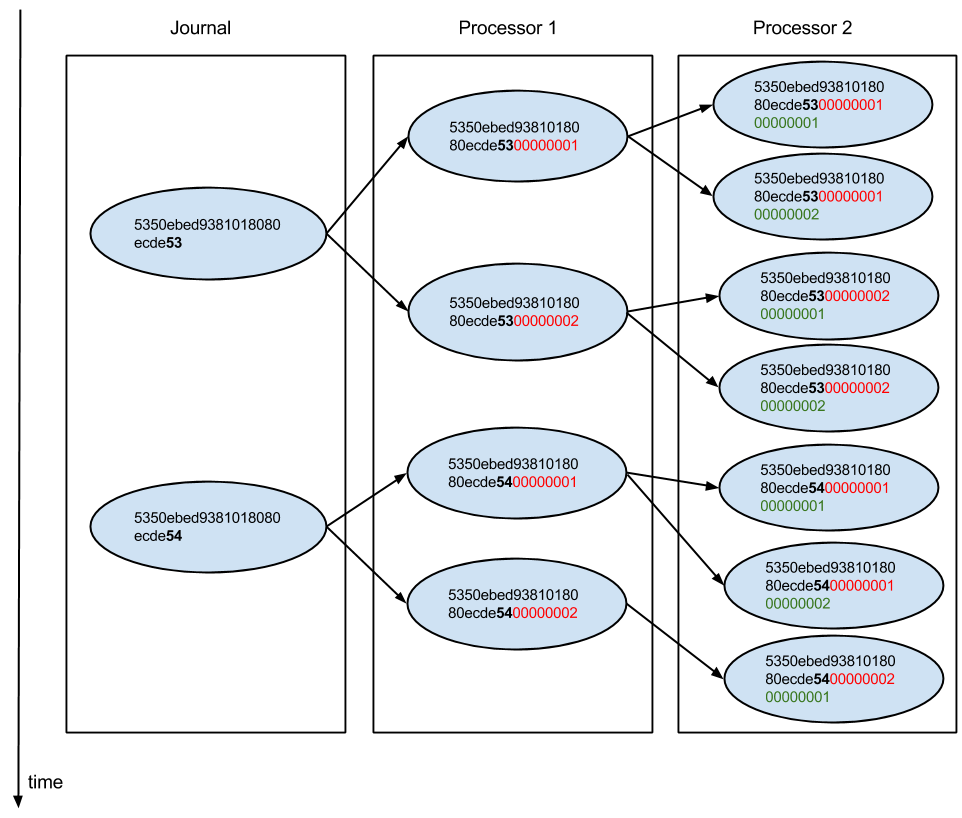
\includegraphics[width=1.0\textwidth]{img/pathidserde.png}}
    \caption{PathId serialization ensuring ordering in MongoDB local journals}
    \label{fig:pathidserde}
  \end{center}
\end{figure}

Listing \ref{lst:pathidserde} shows the code of Path Id and its serialization and deserialization.

\begin{listing}[h]
\begin{minted}[fontsize=\codesize, frame=lines, framesep=2mm]{scala}
case class PathId(rootEvent: String, path: Vector[Int])

object PathId {
  import reactivemongo.bson.utils.Converters
  import java.nio.ByteBuffer

  def apply(rootEvent: String): PathId = PathId(rootEvent, Vector.empty)

  def serialize(id: PathId): String = {
    val array = id.path
    val byteBuffer = ByteBuffer.allocate(array.length * 4)
    val intBuffer = byteBuffer.asIntBuffer
    intBuffer.put(array.toArray)
    byteBuffer.flip()

    id.rootEvent + Converters.hex2Str(byteBuffer.array())
  }

  def deserialize(str: String): PathId = {
    val (idStr, pathStr) = str.splitAt(12*2)

    val byteBuffer = ByteBuffer.allocate(4)
    val arrayBytes = Converters.str2Hex(pathStr)
    val path = arrayBytes.grouped(4).toVector map { bytes =>
      byteBuffer.put(bytes)
      byteBuffer.flip()
      val int = byteBuffer.getInt
      byteBuffer.clear()
      int
    }

    PathId(idStr, path)
  }

  val min = PathId("000000000000000000000000")
}
\end{minted}
\caption{PathId serialization and deserialization}
\label{lst:pathidserde}
\end{listing}


\subsection{Processors}

A stream processor is composed of one Iteratee in input and several Enumerators in output (one per child). 
In order to link the Iteratee with the Enumerators, we use the Promise abstraction to be able to fulfill manually a Future, and Scala STM \footfullcite{bib:scalastm} to handle concurrent accesses on shared state. 

When the Iteratee receives an input event, it processes it to create a substream that is flattened in-place into the main stream using the Enumeratee.mapFlatten helper. Moreover, the Enumeratee updatePathId is responsible of updating the PathId of each sub-event with the new level in the event tree.

Then, each sub-event goes through the effector method that is an Enumeratee executing asynchronously and sequentially the performAtomicSideEffect method (which is the insertion
in the local journal for persistent processors).

Last, sub-events go in the downstreamTrigger Iteratee that updates the state of each child according to the state transition diagram Figure \ref{fig:childstates}. Moreover, each
child that is UpToDate had previously registered a Promise to trigger in the consumersTrigger Map. This promise is linked to a Future that is returned by the Enumerator of a child
when this one is up to date. Thus, when we call promise.trySuccess(Some(outEvent)), the Future pushed in the Enumerator is fulfilled with the new sub-event (and so it will be sent
to the child).
\\

In the Enumerator corresponding to a child (the createOutStream method), when the code is called a new time (corresponding the ACK that previous events has been processed by the child in local mode,
or that the events are at least in the TCP send buffer in distributed mode), we check the state of the child. If it is UpToDate or WaitingForDownStreamAck, we register
a promise to be called when a new event will come in, and we put the Future linked to the promise into the Enumerator. This mechanism allows non-blocking long-polling.
If it is Late, we call the since method the retrieve the past events from the sinceId parameter. If the processor is a persistent stream processor,
it will directly take the past event streams from its MongoDB local journal and returns an Enumerator of it using the ReactiveMongo reactive driver. If the processor is
a side-effect stream processor, it will ask its parent for the past event streams, removing the last node of the path id and then filtering the substream via an offset (as explained in the architecture part). 
Figure \ref{fig:createOutStream} illustrates this mechanism. 

\begin{figure}
  \begin{center} 
    \makebox[\textwidth]{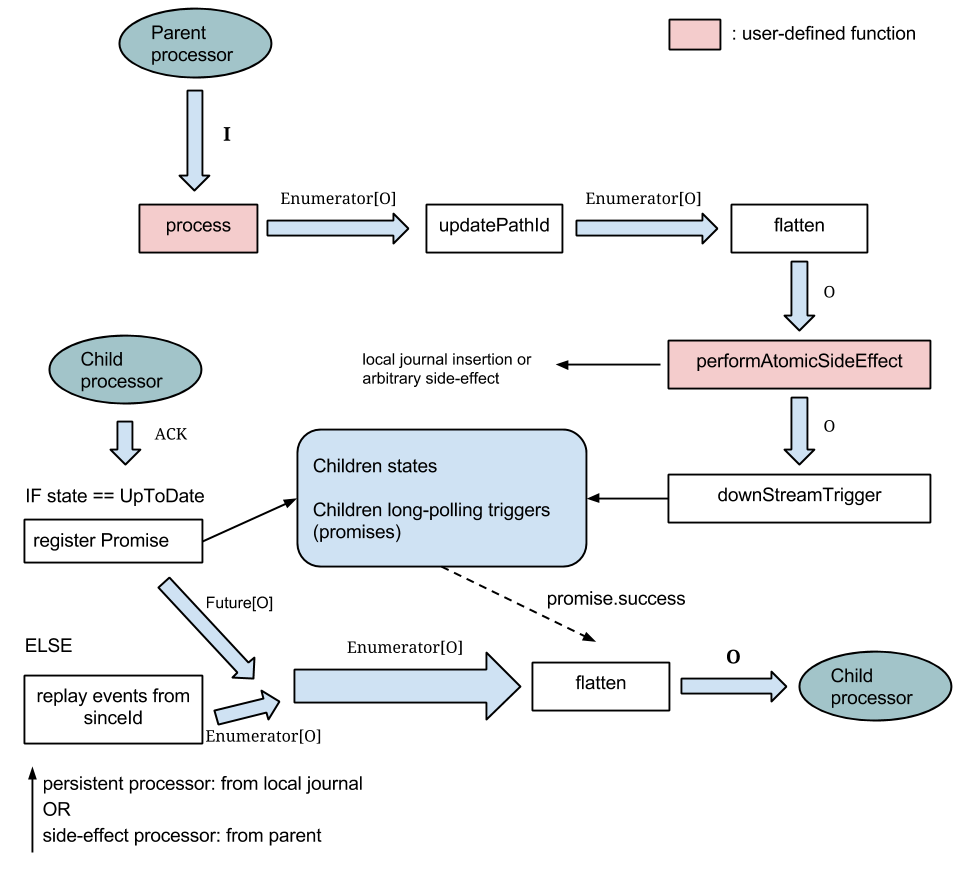
\includegraphics[width=1.0\textwidth]{img/createOutStream.png}}
    \caption{Processor implementation flow}
    \label{fig:createOutStream}
  \end{center}
\end{figure}

In order to share the Maps of Promises and States between the input Iteratee and the output Enumerators (so several concurrent threads), we use Scala STM (Software Transactional Memory) \footfullcite{bib:scalastm}. In a few word, a STM is an optimistic approach to concurrency that let all operations on a shared data structure to be done in parallel. An operation must be committed when it is finished. If there was another commit from another operation during this operation, the operation is aborted (rollback) and tried again. 
Using java.util.concurrent.ConcurrentHashMap is roughly equivalent.

Listing \ref{lst:processor} shows the code of the generic stream processor. Listing \ref{lst:psprocessor} shows the code of persistent stream processor and side-effect stream processor. 
\newpage

\begin{minted}[fontsize=\codesize, frame=lines, framesep=2mm]{scala}
// State for each consumer
sealed trait State
case object UpToDate extends State
case object WaitingForDownStreamAck extends State
case object Late extends State

trait Source[E] {
  def createOutStream(sinceId: PathId): Enumerator[E]
  def since(id: PathId, included: Boolean = false): Enumerator[E]
  def batchQuery(query: JsObject): Enumerator[E] = Enumerator.empty // TOOD: remove default
}

trait Evented[A] {
  def getId(a: A): PathId
  def updateId(a: A, id: PathId): A
  def serialize(a: A): JsObject
}

abstract class StreamProcessor[I, O](implicit ec: ExecutionContext, ei: Evented[I], eo: Evented[O])
   extends Source[O] {
  import scala.concurrent.stm._
  
  def since(id: PathId, included: Boolean = false): Enumerator[O]
  def process(event: I): Enumerator[O]
  def performAtomicSideEffect(event: O): Future[Unit]
  def getLastProcessedEventId(): Future[PathId]
  
  /*
   * Internals
   */

  val consumersTrigger = Ref(Map.empty[String, Promise[Option[O]]])
  val consumersState = Ref(Map.empty[String, State])

  def processor: Enumeratee[I, O] = {
    Enumeratee.mapFlatten[I](inEvent => process(inEvent) &> updatePathId)
  }

  def effector: Enumeratee[O, O] = {
    Enumeratee.mapM[O](outEvent => performAtomicSideEffect(outEvent) map (_ => outEvent))
  }

  def downstreamTrigger: Iteratee[O, Unit] =
    Iteratee.foreach[O] { outEvent =>
      consumersState.single transform { prev =>
        prev mapValues {
          case UpToDate => WaitingForDownStreamAck
          case WaitingForDownStreamAck => Late
          case Late => Late
        }
      }

      val promisesToTrigger = consumersTrigger.single.swap(Map.empty)
      promisesToTrigger foreach { case (_, promise) =>
        promise.trySuccess(Some(outEvent))
      }
    }

  def inStreamSink: Iteratee[I, Unit] = {
    processor ><> effector &>> downstreamTrigger
  }

  def createOutStream(sinceId: PathId): Enumerator[O] = {
    val consumerId = java.util.UUID.randomUUID().toString
    consumersState.single transform (prev => prev + (consumerId -> Late))

    StreamProcessorHelper.unfoldPathId(sinceId) { currentId =>
      val longPollingTrigger = promise[Option[O]]
      consumersTrigger.single.getAndTransform(prev => prev + (consumerId -> longPollingTrigger))

      consumersState.single.get.apply(consumerId) match {
        case WaitingForDownStreamAck | UpToDate =>
          // we are up to date with upstream, no need to pull from source
          consumersState.single.transform(prev => prev + (consumerId -> UpToDate))
          longPollingTrigger.future map { maybeEvent =>
            maybeEvent map (event => Some(currentId, Enumerator(event))) getOrElse 
              Some(currentId, Enumerator.empty[O])
          }

        case Late =>
          StreamProcessorHelper.headOption(since(currentId)) flatMap {
            case (None, _) =>
              // we don't have anything more to poll
              consumersState.single.transform(prev => prev + (consumerId -> UpToDate))
              longPollingTrigger.future map { maybeEvent =>
                maybeEvent map (event => Some(currentId, Enumerator(event))) getOrElse 
                  Some(currentId, Enumerator.empty[O])
              }

            case (Some(event), remainingEnum) =>
              // ignore promise
              consumersTrigger.single.getAndTransform(prev => prev - consumerId)
              // send next events
              Future.successful(Some(currentId, Enumerator(event) andThen remainingEnum))
          }
      }
    }
  }

  def updatePathId: Enumeratee[O, O] = StreamProcessorHelper.mapWithCounter { (outEvent, n) =>
    val oldId = eo.getId(outEvent)
    val newId = oldId.copy(path = oldId.path :+ n)
    eo.updateId(outEvent, newId)
  }
}
\end{minted}
\captionof{listing}{Processor implementation\label{lst:processor}}

\begin{minted}[fontsize=\codesize, frame=lines, framesep=2mm]{scala}
abstract class StreamProcessorWithReplayableSource[I, O]
  (implicit ec: ExecutionContext, ei: Evented[I], eo: Evented[O]) extends StreamProcessor[I, O] {

  val source: Source[I]

  def realtime(sinceId: PathId): Unit = {
    // restart the processor in case of failure
    def loopRestart(futIt: Future[Iteratee[I, Unit]]): Future[Iteratee[I, Unit]] = {
      futIt flatMap { _ =>
        getLastProcessedEventId() flatMap { lastId =>
          loopRestart(source.createOutStream(lastId) |>> inStreamSink)
        }
      }
    }

    loopRestart(source.createOutStream(sinceId) |>> inStreamSink)
  }

  def start(): Future[Unit] = {
    for {
      sinceId <- getLastProcessedEventId()
    } yield realtime(sinceId)
  }

}

abstract class SideEffectStreamProcessor[I, O](implicit ec: ExecutionContext,
    ei: Evented[I], eo: Evented[O]) extends StreamProcessorWithReplayableSource[I, O] {

  def since(id: PathId, included: Boolean = false): Enumerator[O] = {
    val ancestors = id.path.dropRight(1)

    val offset =
      if (id == PathId.min) 0
      else id.path.lastOption.getOrElse(0) + (if (included) 0 else 1)

    source.since(PathId(id.rootEvent, ancestors), included = true) &>
    processor &>
    Enumeratee.drop[O](offset)
  }
}

abstract class PersistentStreamProcessor[I, O](implicit ec: ExecutionContext, 
    ei: Evented[I], eo: Evented[O]) extends StreamProcessorWithReplayableSource[I, O] {

  def collection: JSONCollection
  def performAtomicSideEffect(event: O): Future[Unit] = 
    collection.insert(eo.serialize(event)) map (_ => ())
}
\end{minted}
\captionof{listing}{Persistent processor and side-effect processor implementation\label{lst:psprocessor}}


\subsection{Journal}

The Journal extends StreamProcessor but it differs from other processors by its way of handling input. Indeed, the Journal has multiple pushers (that pull from various data sources) that push events concurrently. To be sure to insert events with an increasing ordered id, we use Concurrent.broadcast that provides a channel to push events. Pushed events will go into an unique sequential pipeline that first creates a PathId for the event, and then insert this event with its PathId to MongoDB (this is done by the journalSink Iteratee). Listing \ref{lst:journalimpl} shows the code of the Journal.

\begin{listing}[h]
\begin{minted}[fontsize=\codesize, frame=lines, framesep=2mm]{scala}
abstract class Journal[E](implicit ec: ExecutionContext, eo: Evented[E]) 
    extends StreamProcessor[E, E] {

  def collection: JSONCollection

  val (enum, channel) = Concurrent.broadcast[(E, Promise[E])]
  
  protected  def journalSink: Iteratee[(E, Promise[E]), Unit] = {
   Enumeratee.mapM[(E, Promise[E])] { case (event, p) =>
     // generate new event id to ensure that event are inserted in ascending order
     val bsonid = BSONObjectID.generate 
     val value = bsonid.value
     value(7) = Byte.MinValue // remove thread id to ensure sequentiality of events
     value(8) = Byte.MinValue
     val eventToInsert = eo.updateId(event, PathId(BSONObjectID(value).stringify))
     collection.insert(eo.serialize(eventToInsert)) map { _ =>
       p.trySuccess(eventToInsert)
       eventToInsert
     }
   } &>> downstreamTrigger
  }

  def start(): Future[Unit] = {
    enum |>> journalSink
    Future.successful()
  }


  def write(event: E): Future[E] = {
    val p = promise[E]
    channel.push(event, p)
    p.future
  }

  def writeSequentially(events: Seq[E]): Future[Option[E]] =
    Enumerator.enumerate(events) |>>> Iteratee.foldM(Option.empty[E]) { (_, event) =>
      write(event) map (Some(_))
    }

  def process(event: E): Enumerator[E] = Enumerator(event)
  override def inStreamSink = Iteratee.ignore // use journalSink instead
  def performAtomicSideEffect(event: E): Future[Unit] = Future.successful(())
  override def updatePathId = Enumeratee.map(identity) // 1 to 1 event generation relationship
}
\end{minted}
\caption{Journal implementation}
\label{lst:journalimpl}
\end{listing}


\subsection{Distribution}

Implementing point-to-point distribution is very easy thanks to Play Framework's helper to transform an Enumerator into an HTTP Stream and HTTP Stream into an Iteratee.

Basically, a parent processor can expose HTTP end-points for 2 functions: \verb|createOutStream| that push the infinite stream, and \verb|since| that allows child side-effect processors to ask for replay of past events.
\verb|createOutStream| can be mapped to an URL like \verb|/stream?pathId=<PATH_ID>| where PathId is the start point of the stream (non-included).
\verb|since| can be mapped to \verb|/since?pathId=<PATH_ID>&included=<BOOLEAN>| where PathId is the start point of the stream and included a boolean stating if we want the event
corresponding to PathId to be replayed. Contrary to \verb|createOutStream|, the since HTTP Stream is not infinite: it finishes when there is no more event to replay.
Listing \ref{lst:remoteparent} shows the implementation of such HTTP interface.

\begin{listing}[h]
\begin{minted}[fontsize=\codesize, frame=lines, framesep=2mm]{scala}
object ProcessorHTTPInterface extends Controller {
  def stream(sinceId: String) = Action {
    val pathId = PathId.deserialize(sinceId)
    val enum = processor.createOutStream(pathId) &> Enumeratee.map(Json.toJson(_))
    Ok.chunked(enum)
  }

  def since(sinceId: String, included: Boolean) = Action {
    val pathId = PathId.deserialize(sinceId)
    val enum = processor.since(pathId, included) &> Enumeratee.map(Json.toJson(_))
    Ok.chunked(enum andThen Enumerator.eof)
  }
}
\end{minted}
\caption{Distributed processors: HTTP interface of a parent processor}
\label{lst:remoteparent}
\end{listing}

Concerning the child processor that has a remote parent, it must declare a remote source of type Source that can be transparently plugged into the StreamProcessor class. Listing \ref{lst:remotechild} shows the implementation of a remote source.

\begin{listing}[h]
\begin{minted}[fontsize=\codesize, frame=lines, framesep=2mm]{scala}
class RemoteParentProcessor extends Source[ZEvent] {
  val remoteParentUrl = "http://localhost:9001"

  def createOutStream(sinceId: PathId): Enumerator[ZEvent] = {
    val serializedId = PathId.serialize(sinceId)
    val url = s"$remoteParentUrl/stream?sinceId=$serializedId"
    getHttpStream(url)
  }

  def since(sinceId: PathId, included: Boolean = false) = {
    val serializedId = PathId.serialize(sinceId)
    val url = s"$remoteParentUrl/since?sinceId=$serializedId&included=$included"
    getHttpStream(url)
  }

  private def getHttpStream(url: String): Enumerator[ZEvent] = {
    val (it, enum) = Concurrent.joined[Array[Byte]]
    WS.url(url).get(_ => it).flatMap(_.run)
    enum &> Enumeratee.mapInput {
      case Input.El(chunk) =>
        val tryJs = Try(Json.parse(chunk))
        tryJs match {
          case Success(js) =>
            js.validate[ZEvent] map { ev =>
              Input.El(ev)
            } getOrElse {
              Input.Empty
            }

          case Failure(err) =>
            logger.error("Failure during json parsing", err)
            Input.Empty
        }

      case Input.Empty => Input.Empty
      case Input.EOF => Input.EOF
    }
  }
}
\end{minted}
\caption{Distributed processors: Remote source implementation of a child processor}
\label{lst:remotechild}
\end{listing}

Composability of Enumerators / Iteratees makes the distribution very easy (almost location transparent). Moreover, as explained in the architecture part, this code maintains
back-pressure with TCP-level ACK, which is very efficient.


\subsection{Example application}

The example application described in the architecture part has been implemented. The major part of the code is business specific and therefore will not be part of the report, but as an example Listing \ref{lst:exampleappimpl} shows the implementation of the FlatSnapshot side-effect processor.

\begin{listing}[h]
\begin{minted}[fontsize=\codesize, frame=lines, framesep=2mm]{scala}
object FlatSnapshot extends SideEffectStreamProcessor[ZEvent, ZEvent] with FlatSnapshotQuery {
  def collection = ReactiveMongoPlugin.db.collection[JSONCollection]("flat_snapshots")

  val logger: LazyLogger = LazyLogger.apply("api.FlatSnapshot")
  
  val source = Snapshot
  
  def getLastProcessedEventId(): Future[PathId] = {
    collection.find(Json.obj(), Json.obj(
      "_lastUpdateByEvent" -> 1)).sort(
      Json.obj("_lastUpdateByEvent" -> -1)).one[JsObject].map(_.flatMap { json =>
        (json \ "_lastUpdateByEvent").asOpt[PathId]
      }.getOrElse(PathId.min))
  }
  
  def process(event: ZEvent): Enumerator[ZEvent] = Enumerator(event)
  
  def performAtomicSideEffect(event: ZEvent): Future[Unit] = {
    val snapshot = ZSnapshot(event)
    if (!(event.body \ "archived").asOpt[Boolean].isEmpty) {
      FlatSnapshot.collection.remove(Json.obj("_id" -> snapshot.id)) map (_ => ())
    } else {
      FlatSnapshot.collection.save(ZSnapshot(event)) map (_ => ())
    }
  }

}
\end{minted}
\caption{Implementation of the FlatSnapshot side-effect processor}
\label{lst:exampleappimpl}
\end{listing}






\newpage
\printbibliography

\newpage
\listoffigures

\newpage
\listoflistings

\end{document}
